\documentclass[border=10pt]{standalone}
\usepackage{tikz}
\usetikzlibrary{arrows.meta, positioning, calc, fit, shapes.geometric}

\begin{document}
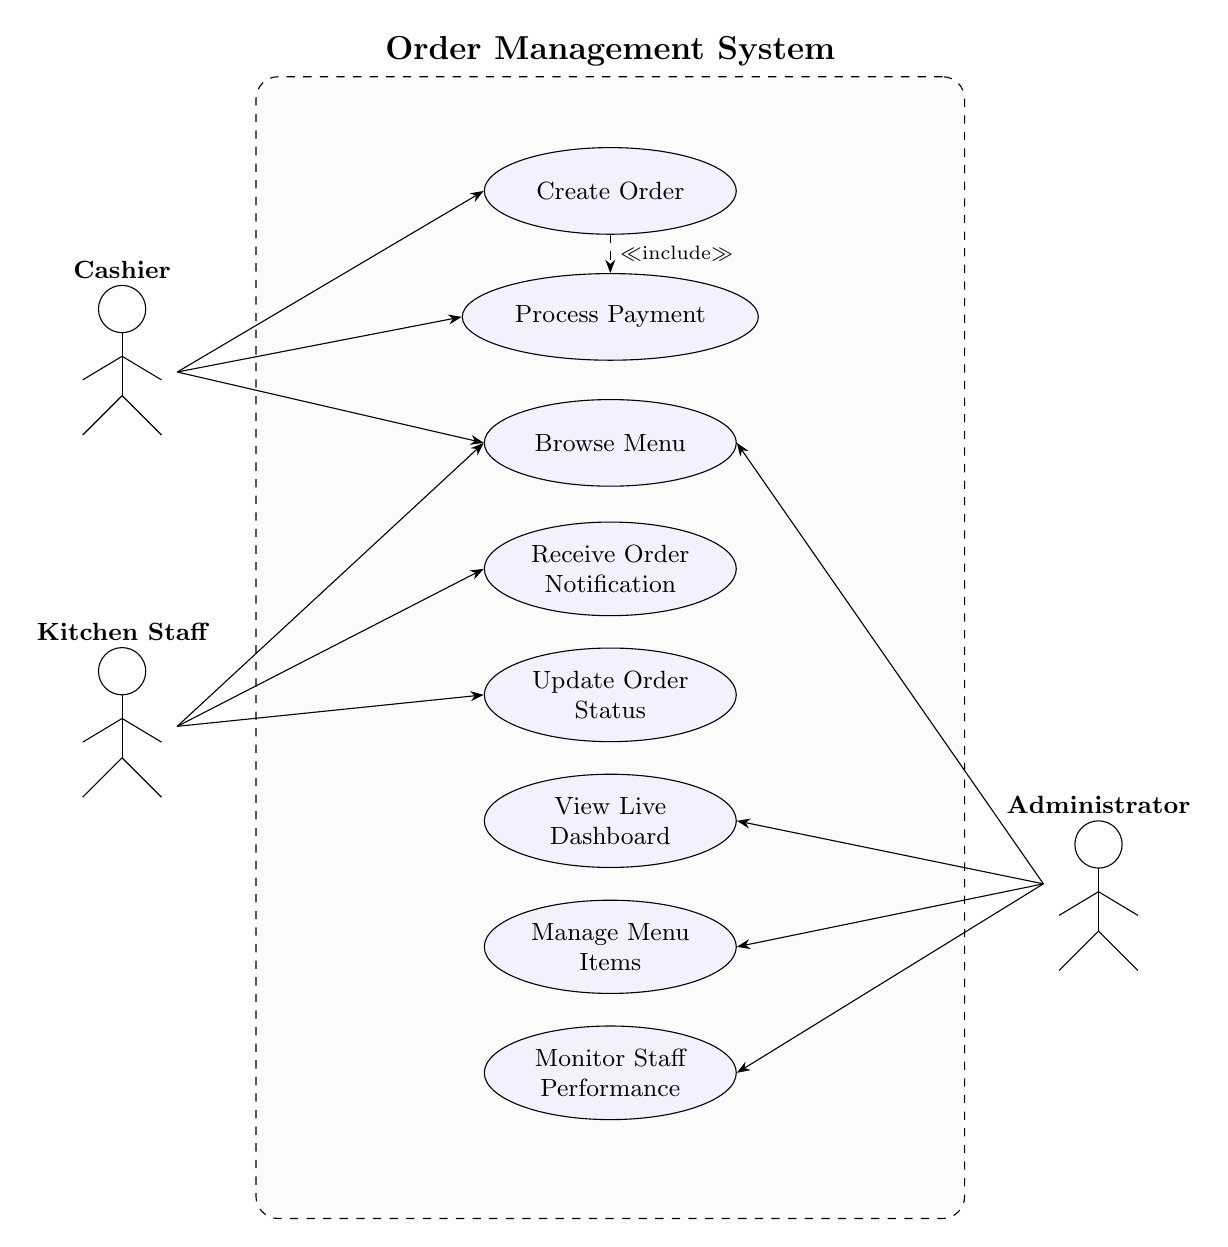
\begin{tikzpicture}[
    actor/.style={draw, minimum width=1.2cm, minimum height=2cm, align=center, font=\small\bfseries},
    usecase/.style={draw, ellipse, minimum width=3.2cm, minimum height=1.1cm, align=center, font=\small, fill=blue!5},
    systembg/.style={draw, dashed, rounded corners=8pt, fill=gray!3, inner sep=12pt},
    >=Stealth
]

% System boundary
\node[systembg, minimum width=9cm, minimum height=14.5cm, label={[font=\large\bfseries]above:Order Management System}] (sys) at (5,0) {};

% Use Cases
\node[usecase] (uc1) at (5, 5.8) {Create Order};
\node[usecase] (uc2) at (5, 4.2) {Process Payment};
\node[usecase] (uc3) at (5, 2.6) {Browse Menu};
\node[usecase] (uc4) at (5, 1.0) {Receive Order\\Notification};
\node[usecase] (uc5) at (5, -0.6) {Update Order\\Status};
\node[usecase] (uc6) at (5, -2.2) {View Live\\Dashboard};
\node[usecase] (uc7) at (5, -3.8) {Manage Menu\\Items};
\node[usecase] (uc8) at (5, -5.4) {Monitor Staff\\Performance};

% Actors - stick figures
% Cashier (left)
\node[font=\small\bfseries] at (-1.2, 4.8) {Cashier};
\draw (-1.2, 4.3) circle (0.3);
\draw (-1.2, 4.0) -- (-1.2, 3.2);
\draw (-1.2, 3.7) -- (-0.7, 3.4);
\draw (-1.2, 3.7) -- (-1.7, 3.4);
\draw (-1.2, 3.2) -- (-0.7, 2.7);
\draw (-1.2, 3.2) -- (-1.7, 2.7);

% Kitchen Staff (left)
\node[font=\small\bfseries] at (-1.2, 0.2) {Kitchen Staff};
\draw (-1.2, -0.3) circle (0.3);
\draw (-1.2, -0.6) -- (-1.2, -1.4);
\draw (-1.2, -0.9) -- (-0.7, -1.2);
\draw (-1.2, -0.9) -- (-1.7, -1.2);
\draw (-1.2, -1.4) -- (-0.7, -1.9);
\draw (-1.2, -1.4) -- (-1.7, -1.9);

% Administrator (right)
\node[font=\small\bfseries] at (11.2, -2.0) {Administrator};
\draw (11.2, -2.5) circle (0.3);
\draw (11.2, -2.8) -- (11.2, -3.6);
\draw (11.2, -3.1) -- (11.7, -3.4);
\draw (11.2, -3.1) -- (10.7, -3.4);
\draw (11.2, -3.6) -- (11.7, -4.1);
\draw (11.2, -3.6) -- (10.7, -4.1);

% Connections - Cashier
\draw[->] (-0.5, 3.5) -- (uc1.west);
\draw[->] (-0.5, 3.5) -- (uc2.west);
\draw[->] (-0.5, 3.5) -- (uc3.west);

% Connections - Kitchen Staff
\draw[->] (-0.5, -1.0) -- (uc4.west);
\draw[->] (-0.5, -1.0) -- (uc5.west);
\draw[->] (-0.5, -1.0) -- (uc3.west);

% Connections - Administrator
\draw[->] (10.5, -3.0) -- (uc6.east);
\draw[->] (10.5, -3.0) -- (uc7.east);
\draw[->] (10.5, -3.0) -- (uc8.east);
\draw[->] (10.5, -3.0) -- (uc3.east);

% Include relationships
\draw[->, dashed] (uc1) -- node[right, font=\scriptsize] {$\ll$include$\gg$} (uc2);

\end{tikzpicture}
\end{document}
